\documentclass[cjk,slidestop,compress,mathserif,blue]{beamer}
%dvipdfm选项是关键,否则编译统统通不过
%beamer的颜色选项定义的是导航条和标题的颜色(即关键词structure的颜色)

%%%%%%%%%%%%%%%%仅限于XeTeX可使用的宏包%%%%%%%%%%%%%%%%%%%%%%%%%%%%
\usepackage{fontspec,xunicode,xltxtra,beamerthemesplit}
%\usepackage{beamerthemesplit}
\usepackage{xeCJK}
\setCJKmainfont[BoldFont=黑体, ItalicFont=楷体, BoldItalicFont=仿宋]{黑体}
%\setsansfont[Mapping=tex-text]{Adobe 黑体 Std}
%如果装了Adobe Acrobat,可在font.conf中配置Adobe字体的路径以使用其中文字体
%也可直接使用系统中的中文字体如SimSun,SimHei,微软雅黑 等
%原来beamer用的字体是sans family;注意Mapping的大小写,不能写错

%%%%%%%%   确定标题和导航条结构的框架     %%%%%%%%%%%%
\usepackage{beamerthemeshadow}                       %
%\usepackage{beamerthemeclassic}%导航条色与背景色一致%
%%%%%%%%%%%%%%%%%%%%%%%%%%%%%%%%%%%%%%%%%%%%%%%%%%%%%%
\setbeamerfont{roman title}{size={}}
%\usepackage{CJK} % CJK 中文支持                                  %
\usepackage{amsmath,amsthm,amsfonts,amssymb,bm}
\usepackage{mathrsfs}
\usepackage{xcolor}                                        %使用默认允许使用颜色
\usepackage{hyperref} 
\usepackage{graphicx}
\usepackage{subfigure}           %图片跨页
\usepackage{caption}
\captionsetup{font=footnotesize}

\usepackage{multirow}

%\usepackage[numbers,sort&compress]{natbib} %紧密排列             %
\usepackage[sectionbib]{chapterbib}        %每章节单独参考文献   %
\usepackage{hypernat}                                                                         %
%\usepackage[dvipdfm,bookmarksopen=true,pdfstartview=FitH,CJKbookmarks]{hyperref}		%
\hypersetup{bookmarksnumbered,colorlinks,linkcolor=brown,citecolor=blue,urlcolor=red}         %
%参考文献含有超链接引用时需要下列宏包,注意与natbib有冲突        %
%\usepackage[dvipdfm]{hyperref}                                  %
%\usepackage{hypernat}                                           %
\newcommand{\upcite}[1]{\hspace{0ex}\textsuperscript{\cite{#1}}} %

%\useoutertheme{smoothbars}
\useinnertheme[shadow=true]{rounded}
\usetheme{Berkeley}                                          %主题式样
%\usetheme{Luebeck}

\usecolortheme{lily}                                        %颜色主题式样

\usefonttheme{professionalfonts}                           %字体主题样式宏包

%\beamertemplatetransparentcoveredhigh                      %使所有被隐藏的文本高度透明
\beamertemplatetransparentcovereddynamicmedium             %使所有被隐藏的文本完全透明,动态,动态的范围很小
\mode<presentation>
%\beamersetaveragebackground{gray}                          %设置背景颜色(单一色) 
\beamertemplateshadingbackground{green!10}{red!5}         %设置背景颜色(渐变色)

%在指定位置精确放置logo
\usepackage{tikz}
\usepackage{beamerfoils}
\usepackage{pgf}
\logo{\pgfputat{\pgfxy(11.68,0.15)}{
\includegraphics[height=1.01cm,viewport=0 0 140 120,clip]{Figures/BCC_logo-1.png}}\pgfputat{\pgfxy(10.502,-0.218)}{
\includegraphics[height=0.369cm,viewport=140 0 540 120,clip]{Figures/BCC_logo-1.png}}}
%\logo{\pgfputat{\pgfxy(11.68,0.15)}{
\includegraphics[height=0.95cm,viewport=0 0 510 360,clip]{Figures/Logo_Gainstrong.png}}\pgfputat{\pgfxy(10.333,-0.195)}{
\includegraphics[height=0.35cm,viewport=530 70 1100 218,clip]{Figures/Logo_Gainstrong.png}}}
%\MyLogo{
%	\pgfputat{\pgfxy(-50,-50)}{\pgfbox[right,base]{
\includegraphics[height=1cm]{Figures/BCC_logo-1.png}}}

%logo作为背景放置
%\setbeamertemplate{background}{
%	\pgfputat{\pgfxy(6.5,-0.5)}{\pgfbox[left,top]{\pgfimage[height=1.1cm]{Figures/BCC_logo-1.png}}}}

%\logo{}									%不显示logo

\begin{document}
%\begin{CJK*}{GBK}{song}
%\begin{CJK*}{GBK}{kai}
%beamer下不能用\songyi、\zihao等命令!
%\graphicspath{Figures/}

%-------------------------------PPT Title-------------------------------------
\title{k空间布点与积分(三)}
%-----------------------------------------------------------------------------

%----------------------------Author & Date------------------------------------
\author{北京市计算中心\;云平台\:姜骏}
\date{\textrm{2016.11.23}}
%\date{2013.09.10}
\frame{\titlepage}
%-----------------------------------------------------------------------------

%------------------------------------------------------------------------------列出全文 outline ---------------------------------------------------------------------------------
\section*{}
\frame[allowframebreaks]
{
  \frametitle{Outline}
%  \frametitle{\textcolor{mycolor}{\secname}}
  \tableofcontents%[current,currentsection,currentsubsection]
}
%在每个section之前列出全部Outline
%类似的在每个subsection之前列出全部Outline是\AtBeginSubsection[]
\AtBeginSection[]
{
  \frame<handout:0>
  {
    \frametitle{Outline}
%全部Outline中,本部分加亮
    \tableofcontents[current,currentsection]
  }
}

%------------------------------------------------------------------------------PPT main Body------------------------------------------------------------------------------------
\small
\section{导体的\rm{Fermi}面与展宽}
\frame
{
	\frametitle{导体的\textrm{Fermi}~面与展宽}
	\begin{itemize}
		\item 由于导体的\textrm{Fermi}~面穿过某些能带,因此被积函数在\textrm{Fermi}~面上是不连续的,积分随$\vec k$~点收敛很慢
		\item 引入含有展宽\textrm{(smearing)}参数$W$的分布函数(如\textrm{Gaussian~}、\textrm{Lorentz~}等函数)可以有效地提升导体在\textrm{Fermi~}面附近的$\vec k$~点收敛性
	\end{itemize}
	计算积分
	$$I=\int_{\mathrm{BZ}}S(E(\vec k)-E_{\mathrm F})f(\vec k)\mathrm{d}\vec k=\int_{-\infty}^{\infty}S(\varepsilon-E_{\mathrm F})f(\varepsilon)\mathrm{d}\varepsilon$$
	这里$$F(\varepsilon)=\int_{\mathrm{BZ}}f(\vec k)\delta(\varepsilon-E(\vec k))\mathrm{d}\vec k$$
	$E(\vec k)$是能带的色散关系,$E_{\mathrm F}$是\textrm{Fermi~}能级,$f(\vec k)$~是被积函数
	\begin{displaymath}
		S(x)=1-\theta(x)=\left\{
		\begin{aligned}
			1\quad x\leqslant0\\
			0\quad x>0
		\end{aligned}\right.
	\end{displaymath}
}

\frame
{
	\frametitle{导体的\textrm{Fermi}~面与展宽}
	当\textrm{step~}函数$S(x)$用\textrm{Fermi-Dirac}分布函数代替,可以很好地提升$\vec k$~点收敛性,但因此引入了误差
	\begin{figure}[h!]
	\centering
	\vspace*{-0.2in}
	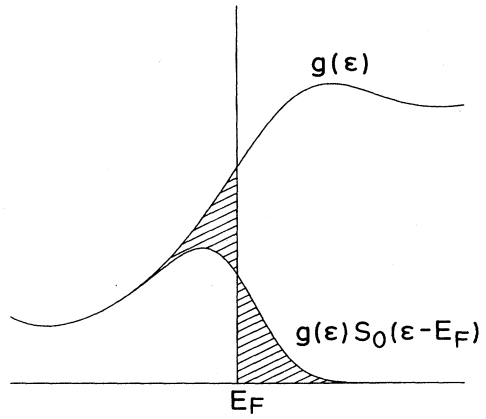
\includegraphics[height=1.1in,width=1.25in,viewport=0 0 530 500,clip]{Figures/MP_distribution.png}
	\caption{\textrm{A schematic density of states $g(\varepsilon)$ and function multiplied by a smooth distribution function.}}%
	\label{MP_distribution}
	%\hspace*{-10pt}
	\end{figure} 
	\textrm{Methfessel-Paxton~}提出用更复杂的多项式函数$S_N$\upcite{PRB40-3616_1989},引入变量$x=(\varepsilon-E_{\mathrm F})/W$,为了用函数$S_N(x)$逼近\textrm{Step~}函数$S(x)$,%,并要求$S_N$是平滑函数
	先用\textrm{Hermite~}多项式展开$\delta(x)$
	\vspace*{-8pt}
	\begin{displaymath}
		\delta(x)=\sum_{n=0}^{\infty}A_nH_{2n}(x)\mathrm{e}^{-x^2}
	\end{displaymath}
}

\frame
{
	\frametitle{导体的\textrm{Fermi}~面与展宽}
	利用\textrm{Hermite~}多项式的正交性和\textrm{Gaussian~}权重
	\begin{displaymath}
		\int_{-\infty}^{\infty}H_n(x)H_m(x)\mathrm{e}^{-x^2}\mathrm{d}x=n!2^n\sqrt{\pi}\delta
	\end{displaymath}
	可得系数$A_n$
	\begin{displaymath}
		A_n=\frac{H_{2n}(0)}{(2n)!4^n\sqrt{\pi}}=\frac{(-1)^n}{n!4^n\sqrt{\pi}}
	\end{displaymath}
	因此有$\delta$函数的逼近函数
	\begin{displaymath}
		D_N(x)=\sum_{n=0}^NA_nH_{2n}(x)\mathrm{e}^{-x^2}
	\end{displaymath}
	由此得到\textrm{Step}~函数的逼近函数
	\begin{displaymath}
		S_N(x)=1-\int_{-\infty}^xD_N(t)\mathrm{d}t
	\end{displaymath}
}

\frame
{
	\frametitle{逼近函数}
	利用等式$$\frac{\mathrm d}{{\mathrm d}x}[H_n(x)\mathrm{e}^{-x^2}]=-H_{n+1}(x){\mathrm e}^{-x^2}$$
	\begin{figure}[h!]
		\begin{minipage}[t]{0.55\linewidth}
			可得\textrm{Methfessel-Paxton~}积分
		\begin{displaymath}
			\begin{aligned}
				S_0(x)&=\frac12\left[1-\mathrm{erf}(x)\right]\\
				S_N(x)&=S_0(x)+\sum_{n=1}^NA_nH_{2n-1}(x)\mathrm{e}^{-x^2}
			\end{aligned}
		\end{displaymath}
		\textcolor{blue}{$S_0$对应于\textrm{Gaussian}分布函数}(类似\textrm{Fermi-Dirac}分布函数)
		\end{minipage}
		\hfill
		\begin{minipage}[t]{0.40\linewidth}
		\centering
		\vspace*{-0.8in}
%		\hspace*{0.5in}
		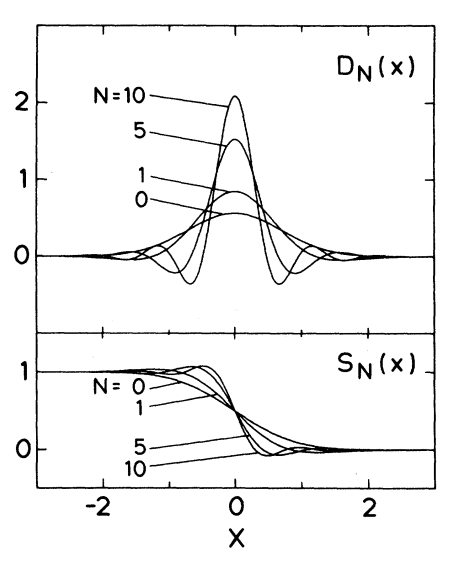
\includegraphics[height=2.0in,width=1.25in,viewport=0 0 530 800,clip]{Figures/MP_SN_DN.png}
		\caption{\textrm{Sucessive approximants to the $\delta$ function, $D_N$ and to the step function $S_N$.}}%
		\label{MP_SN_DN}
		%\hspace*{-10pt}
		\end{minipage}
	\end{figure} 
	\textrm{Methfessel-Paxton~}提出用更复杂的多项式函数$S_N$,引入变量$x=(\varepsilon-E_{\mathrm F})/W$,为了用函数$S_N(x)$逼近\textrm{Step~}函数$S(x)$,%,并要求$S_N$是平滑函数
}

\frame
{
	\frametitle{逼近函数的属性}
	如果有不多于\textrm{2N+1~}项的多项式$P(x)$
	\begin{displaymath}
		\int_{-\infty}^{\infty}D_N(x)P(x)\mathrm{d}x=\int_{-\infty}^{\infty}\delta(x)P(x)\mathrm{d}x=P(0)
	\end{displaymath}
	因此$P(x)$可以用\textrm{Hermite}多项式展开
\begin{itemize}
	\item \begin{displaymath}
			0=\int_{-\infty}^{\infty}\left[D_N(x)-\delta(x)\right]P(x)\mathrm{d}x
	\end{displaymath}
	\item \begin{displaymath}
			0=\int_{-\infty}^{\infty}\left[S_N(x)-S(x)\right]P(x)\frac{{\mathrm d}}{\mathrm dx}\mathrm{d}x
	\end{displaymath}
\end{itemize}
可见$S_N(x)$是对\textrm{Step}函数$S(x)$的很好逼近,当$F(x)$可用不多于\textrm{2N+1~}项多项式表示,则积分误差
$$\int\left[S_N(x)-S(x)\right]F(x)\mathrm{d}x\sim\textcolor{red}{\mathrm{e}^{-x^2}}$$
}

\section{四面体布点与积分方法}
\frame
{
	\frametitle{\textrm{Fermi}面的确定}
	已知每个四面体对积分态密度(态数目)$n_T(\varepsilon)$的贡献
	\begin{itemize}
	\item $\varepsilon<\varepsilon_1$
%		\begin{displaymath}
		\:	$n_T(\varepsilon)=0$
%		\end{displaymath}
	\item $\varepsilon_1<\varepsilon<\varepsilon_2$
%		\begin{displaymath}
		\:	$n_T(\varepsilon)=\dfrac{V_T}{V_G}\dfrac{(\varepsilon-\varepsilon_1)^3}{\varepsilon_{21}\varepsilon_{31}\varepsilon_{41}}$
%		\end{displaymath}
	\item $\varepsilon_2<\varepsilon<\varepsilon_3$
		\begin{displaymath}
			\hspace*{-35pt}	n_T(\varepsilon)=\dfrac{V_T}{V_G}\dfrac1{\varepsilon_{31}\varepsilon_{41}}\left[\varepsilon_{21}^2+3\varepsilon_{21}(\varepsilon-\varepsilon_2)+3(\varepsilon-\varepsilon_2)^2-\dfrac{\varepsilon_{31}+\varepsilon_{42}}{\varepsilon_{32}\varepsilon_{42}}(\varepsilon-\varepsilon_2)^3\right]
		\end{displaymath}
	\item $\varepsilon_3<\varepsilon<\varepsilon_4$
%		\begin{displaymath}
		\:	$n_T(\varepsilon)=\dfrac{V_T}{V_G}\left[1-\dfrac{(\varepsilon_4-\varepsilon)^3}{\varepsilon_{41}\varepsilon_{42}\varepsilon_{43}}\right]$
%		\end{displaymath}
	\item $\varepsilon>\varepsilon_4$
%		\begin{displaymath}
		\:	$n_T(\varepsilon)=\frac{V_T}{V_G}$
%		\end{displaymath}
	\end{itemize}
	利用等能面的插值,由约束条件确定\textrm{Fermi}能级$\varepsilon_{\mathrm F}$
	$$\int_{\varepsilon_0}^{\varepsilon_{\mathrm F}}\sum_{T=1}^{N_{Tet}}n_T(\varepsilon)\mathrm{d}\varepsilon=N_e$$
}

\frame
{
	\frametitle{四面体积分的误差}
	四面体积分的误差有两个来源
	\begin{itemize}
		\item 四面体内的线性插值引入的误差
		\item 四面体内等能面线性插值逼近真实\textrm{Fermi~}面引入的误差
	\end{itemize}
\begin{figure}[h!]
\centering
\vspace*{-0.28in}
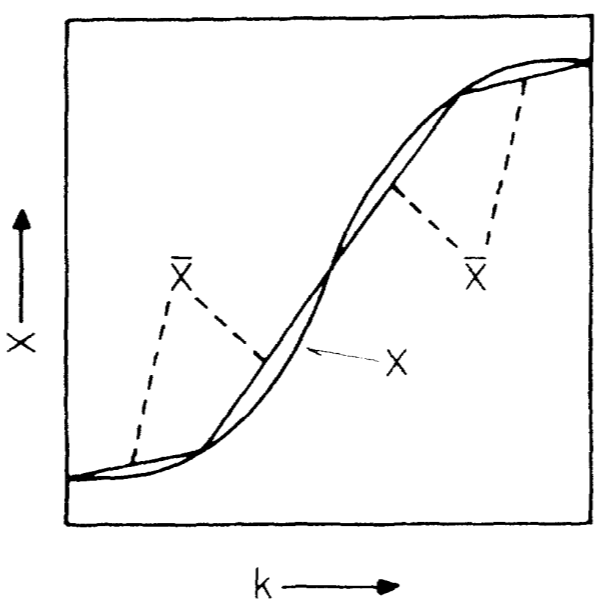
\includegraphics[height=1.25in,width=1.25in,viewport=0 0 650 650,clip]{Figures/Tetra_error.png}
\caption{\small Schematic representation of the interpolation error due to line interpolation.}%(与文献\cite{EPJB33-47_2003}图1对比)
\label{Fig:Tetra_error}
\end{figure}
\textcolor{blue}{对半导体和绝缘体,由于价带被完全填充,用\textrm{Monkhorst-Pack~}布点产生四面体积分方案,可以保证积分误差完全抵消}
}

\frame
{
	\frametitle{四面体积分的误差估计}
		对导体材料,每个四面体内的线性插值积分误差
	\begin{displaymath}
		\delta\langle X\rangle_T=\int_T\mathrm{d}^3k\left[ X(\vec k)-\bar X(\vec k) \right]
	\end{displaymath}
为估计积分误差,假设有被积函数
$$X(\vec k)=a+\sum_ib_ik_i+\frac12\sum_{ij}k_ic_{ij}k_j$$
四面体的一个顶点置于原点,其余三个点位于$\vec t_i=(t_{1i},t_{2i},t_{3i})$,其中$i=1,2,3$
\begin{figure}[h!]
\centering
\vspace*{-0.3in}
\includegraphics[height=1.65in,width=1.70in,viewport=15 15 500 550,clip]{Figures/Brillouin-Tetra.eps}
%\caption{\small .}%(与文献\cite{EPJB33-47_2003}图1对比)
\label{Fig:Tetrahedron}
\end{figure}
}

\frame
{
	\frametitle{四面体积分的误差估计}
变换坐标系$s_i$
$$k_i=\sum_jt_{ij}s_j$$
因此被积函数变换为
$$X(\vec s)=\bar a+\sum_i\bar b_is_i+\frac12\sum_{ij}s_i\bar c_{ij}s_j$$
这里系数$\bar a=a$,$\bar b_i=\sum\limits_jb_jt_{ji}$,$\bar c_{ij}=\sum\limits_{kl}t_{kl}c_{kl}t_{lj}$\\
并且$s_i>0\;i=1,2,3$,$\sum\limits_{i=1}^3s_i\leqslant1$

因此可有被积函数的线性插值为
$$\bar X(\vec s)=\bar a+\sum_i(\bar b_i+\frac12\bar c_{ii})s_i$$
}

\frame
{
	\frametitle{四面体积分的误差估计}
	因此积分误差可以解析表示为
	\begin{displaymath}
		\begin{aligned}
			\delta\langle X\rangle_T=&\mathrm{det}|t_{ij}|\int_T\mathrm{d}^3s\frac12\left[ \sum_{ij}s_i\bar c_{ij}s_j-\sum_i\bar c_{ii}s_i \right]\\
			=&\frac16\mathrm{det}|t_{ij}|\frac1{40}\left[ \sum_{i\neq j}\bar c_{ij}-3\sum_i\bar c_{ii} \right]
		\end{aligned}
	\end{displaymath}
	将$c_{ij}$用被积函数的二阶导数表示,$\frac16\mathrm{det}|t_{ij}|$是四面体体积$V_T$,因此可有
	\begin{displaymath}
		\delta\langle X\rangle_T=V_T\sum_{ij}\left\langle\frac{\partial^2X}{\partial k_i\partial k_j}\right\rangle_TC_{ii}\Delta^2
	\end{displaymath}
	这里$\Delta=\sqrt^3{\mathrm{det}|t|}$
	$$C_{ij}=\frac1{40\Delta^2}\left[ \sum_{l\neq m}t_{il}t_{jm}-3\sum_lt_{ij}t_{jl} \right]$$
}

\frame
{
	\frametitle{四面体积分的误差估计}
	对全部占据四面体误差$\delta\langle X\rangle_T$求和,得到插值误差
	\begin{displaymath}
		\delta\langle X\rangle=\left\langle\sum_{ij}\frac{\partial^2X}{\partial k_i\partial k_j}C_{ii}\right\rangle\Delta^2
	\end{displaymath}
	因此\textcolor{red}{四面体积分误差随$\Delta^2$收敛}

	\textcolor{blue}{根据\textrm{Green's~}积分公式,可将体相积分变成\textrm{Fermi~}面的表面积分}
	\begin{displaymath}
		\begin{aligned}
			\delta\langle X\rangle=&\frac1{V_G}\sum_{ij}\langle C_{ij}\rangle\int_{V_G}\mathrm{d}^3k\frac{\partial^2X}{\partial k_i\partial k_j}\Delta^2\\
			=&\frac1{V_G}\sum_{ij}\langle C_{ij}\rangle\oint_{\varepsilon=\varepsilon_{\mathrm F}}\mathrm{d}^2A_i\frac{\partial X}{\partial k_j}\Delta^2
		\end{aligned}
	\end{displaymath}
因此可有
	\begin{displaymath}
			\delta\langle X\rangle=\frac1{V_G}\sum_{ij}\oint_{\varepsilon=\varepsilon_{\mathrm F}}\mathrm{d}^2A_iC_{ij}\frac{\partial X}{\partial k_j}\Delta^2
	\end{displaymath}
}

\frame
{
	\frametitle{四面体积分的误差}
\vspace*{-10pt}
	将如下关系
	\begin{displaymath}
		\begin{aligned}
		&\int\mathrm{d}^2A_i=\int\mathrm{d}^2|A|\frac1{\nabla_k\varepsilon}\frac{\partial\varepsilon}{\partial k_i}\\
		&\sum_i\frac{\partial\varepsilon}{\partial k_i}t_{ij}=\varepsilon_{j+1}-\varepsilon_1\\
		&\sum_i\frac{\partial X}{\partial k_i}t_{ij}=X_{j+1}-X_1 
		\end{aligned}
	\end{displaymath}
这里$\varepsilon_i$和$X_i$是四面体顶点的能量和被积函数值,
\vspace*{-5pt}
\begin{displaymath}
	\begin{aligned}
		\delta\langle X\rangle=&\sum_TD_T(\varepsilon_{\mathrm F})\frac1{40}\left[\sum_{i\neq j}(X_{i+1}-X_1)(\varepsilon_{j+1}-\varepsilon_1)\right.\\
			&-3\left.\sum_i(X_{i+1}-X_1)(\varepsilon_{j+1}-\varepsilon_1)\right]\\
			=&\sum_TD_T(\varepsilon_{\mathrm F})\frac1{40}\sum_{i=1}^4X_i\sum_{j=1}^4(\varepsilon_j-\varepsilon_i) 
	\end{aligned}
\end{displaymath}
}

\frame
{
	\frametitle{四面体积分权重校正}
	\textcolor{red}{四面体积分权重校正为}
\begin{displaymath}
	\mathrm{d}w_i=\frac{\delta\langle X\rangle}{\delta X_i}=\sum_T\frac1{40}D_T(\varepsilon_{\mathrm F})\sum_{j=1}^4(\varepsilon_j-\varepsilon_i) 
\end{displaymath}

类似地,考虑等能面线性插值对\textrm{Fermi~}面逼近引起的误差,可得\\\textcolor{blue}{每个四面体的电子数校正}
\begin{displaymath}
	\delta N_{\mathrm{el},T}=\frac{A_T}{V_G}\sum_{ij}\frac{\partial^2k_{\mathrm F}}{\partial k_i\partial k_j}C_{ij}\Delta^2
\end{displaymath}
这里$A_T$是三角形面积
	$$C_{ij}=\frac1{24\Delta^2}\left[ \sum_{l\neq m}t_{il}t_{jm}-2\sum_lt_{ij}t_{jl} \right]$$
	其中$t_{ij}$是与四面体类似的三角形顶点适量\\
	\textcolor{red}{对均匀电子,四面体积分误差随$\Delta^3$收敛}
}

\frame
{
	\frametitle{四面体积分的积分权重与展宽}
	\textcolor{red}{四面体$W=\dfrac{\mathrm{d}w_i}{\mathrm{d}\varepsilon}$对能量导数对应于“展宽”}
\begin{figure}[h!]
\centering
\vspace*{-0.28in}
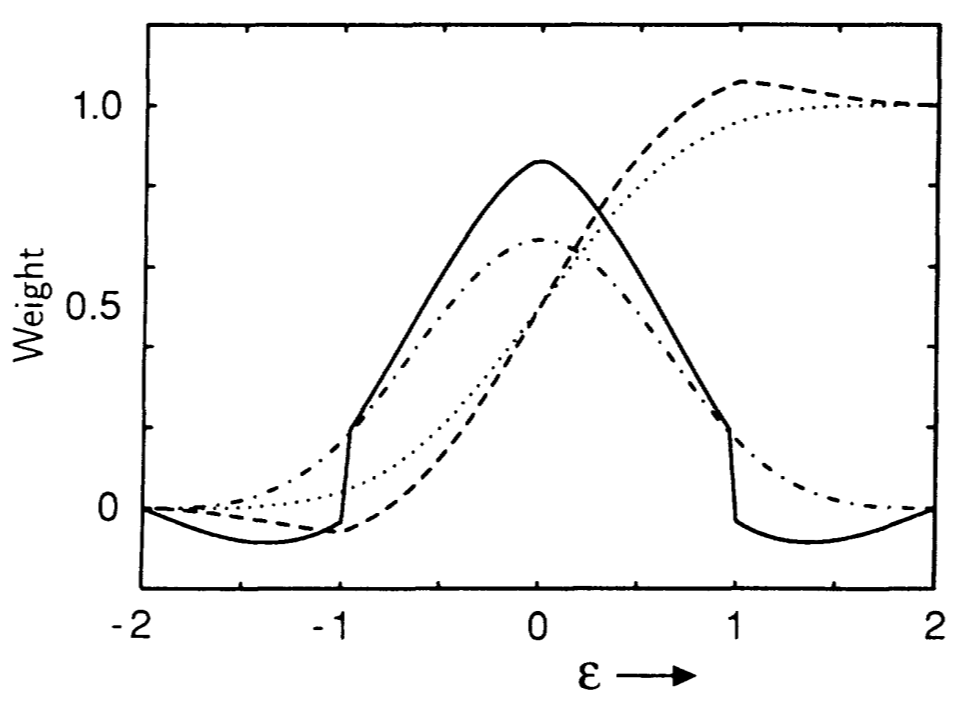
\includegraphics[height=1.4in,width=1.55in,viewport=0 0 1000 800,clip]{Figures/Tetra_smearing.png}
%\caption{\small .}%(与文献\cite{EPJB33-47_2003}图1对比)
\label{Fig:Tetrahedron}
\end{figure}
\begin{itemize}
\vspace*{-0.1in}
	\item \textcolor{blue}{四面体方法展宽参数可随能带分布和形状\\
	传统展宽方法的展宽系数对所有能带都相同}
	\item \textcolor{red}{四面体方法不推荐引入展宽参数}\\
		\begin{enumerate}
			\item 展宽计算的总能不满足变分原理,\textrm{Hellmann-Feynman}定理不再满足,\textcolor{red}{不能正确计算导体的受力}
			\item 四面体能保证态密度计算在\textrm{van Hove}奇点附近出现振荡,引入展宽会破坏这一特征
		\end{enumerate}
\end{itemize}
}

\frame
{
	\frametitle{各种$\vec k$~空间积分方法的比较}
\vskip -7pt
\begin{footnotesize}
\arrayrulewidth=0.4pt
\doublerulesep=0.4pt
\begin{table}[!h]
\tabcolsep 0pt \vspace*{-12pt}
%\begin{minipage}{\textwidth}
\label{tab:magno-1}
\centering
\def\temptablewidth{1.01\textwidth}
{\rule{\temptablewidth}{0.8pt}}
\begin{tabular*} {\temptablewidth}{|c@{\extracolsep{\fill}}|c|c|c|c|}
	\multirow{3}{*}{\textcolor{red}{积分方案}}	&\multicolumn{4}{c|}{\textcolor{blue}{布点方案}:~\textrm{Monkhorst-Pack}~方法} \\\cline{2-5}
	&\multirow{2}{*}{\textrm{Fermi-Dirac}~方法} &\multicolumn{2}{c|}{\textrm{Methfessel-Paxton}~方法} &\multirow{2}{*}{\textrm{Tetrahedron}~方法}\\\cline{3-4}
& &\textrm{Gaussian~} &$N>0$ & \\ \hline
半导体、&\multirow{2}{*}{\textcolor{blue}{$\texttimes$}} &$\delta\leqslant0.05$ &\multirow{2}{*}{\textcolor{red}{$\texttimes$}} &\textcolor{blue}{\textrm{DOS \& total-Energy}}\\
绝缘体 & &\textcolor{blue}{$\checkmark$} & &\textcolor{red}{$\checkmark$} \\\hline
导体、 & \multirow{2}{*}{\textcolor{blue}{$\checkmark$}} & \multicolumn{2}{c|}{\textcolor{blue}{\textrm{Phonon \& relaxation}}} &\textcolor{blue}{\textrm{DOS \& total-Energy}} \\
金属 & &\multicolumn{2}{c|}{\textcolor{red}{$\checkmark$}}  &\textcolor{red}{$\checkmark$} \\\hline
\textrm{supercell} &\multirow{2}{*}{\textcolor{blue}{$\checkmark$}} &\multicolumn{2}{c|}{\multirow{2}{*}{\textcolor{red}{$\checkmark$}}} &\multirow{2}{*}{\textcolor{red}{$\texttimes$}}\\
& &\multicolumn{2}{c|}{} &\\
\end{tabular*}
{\rule{\temptablewidth}{1pt}}\\
%\end{center}1
%\end{minipage}
\end{table}
\end{footnotesize}
}
%\frame
%{
%\begin{figure}[h!]
%\centering
%\vspace*{-0.25in}
%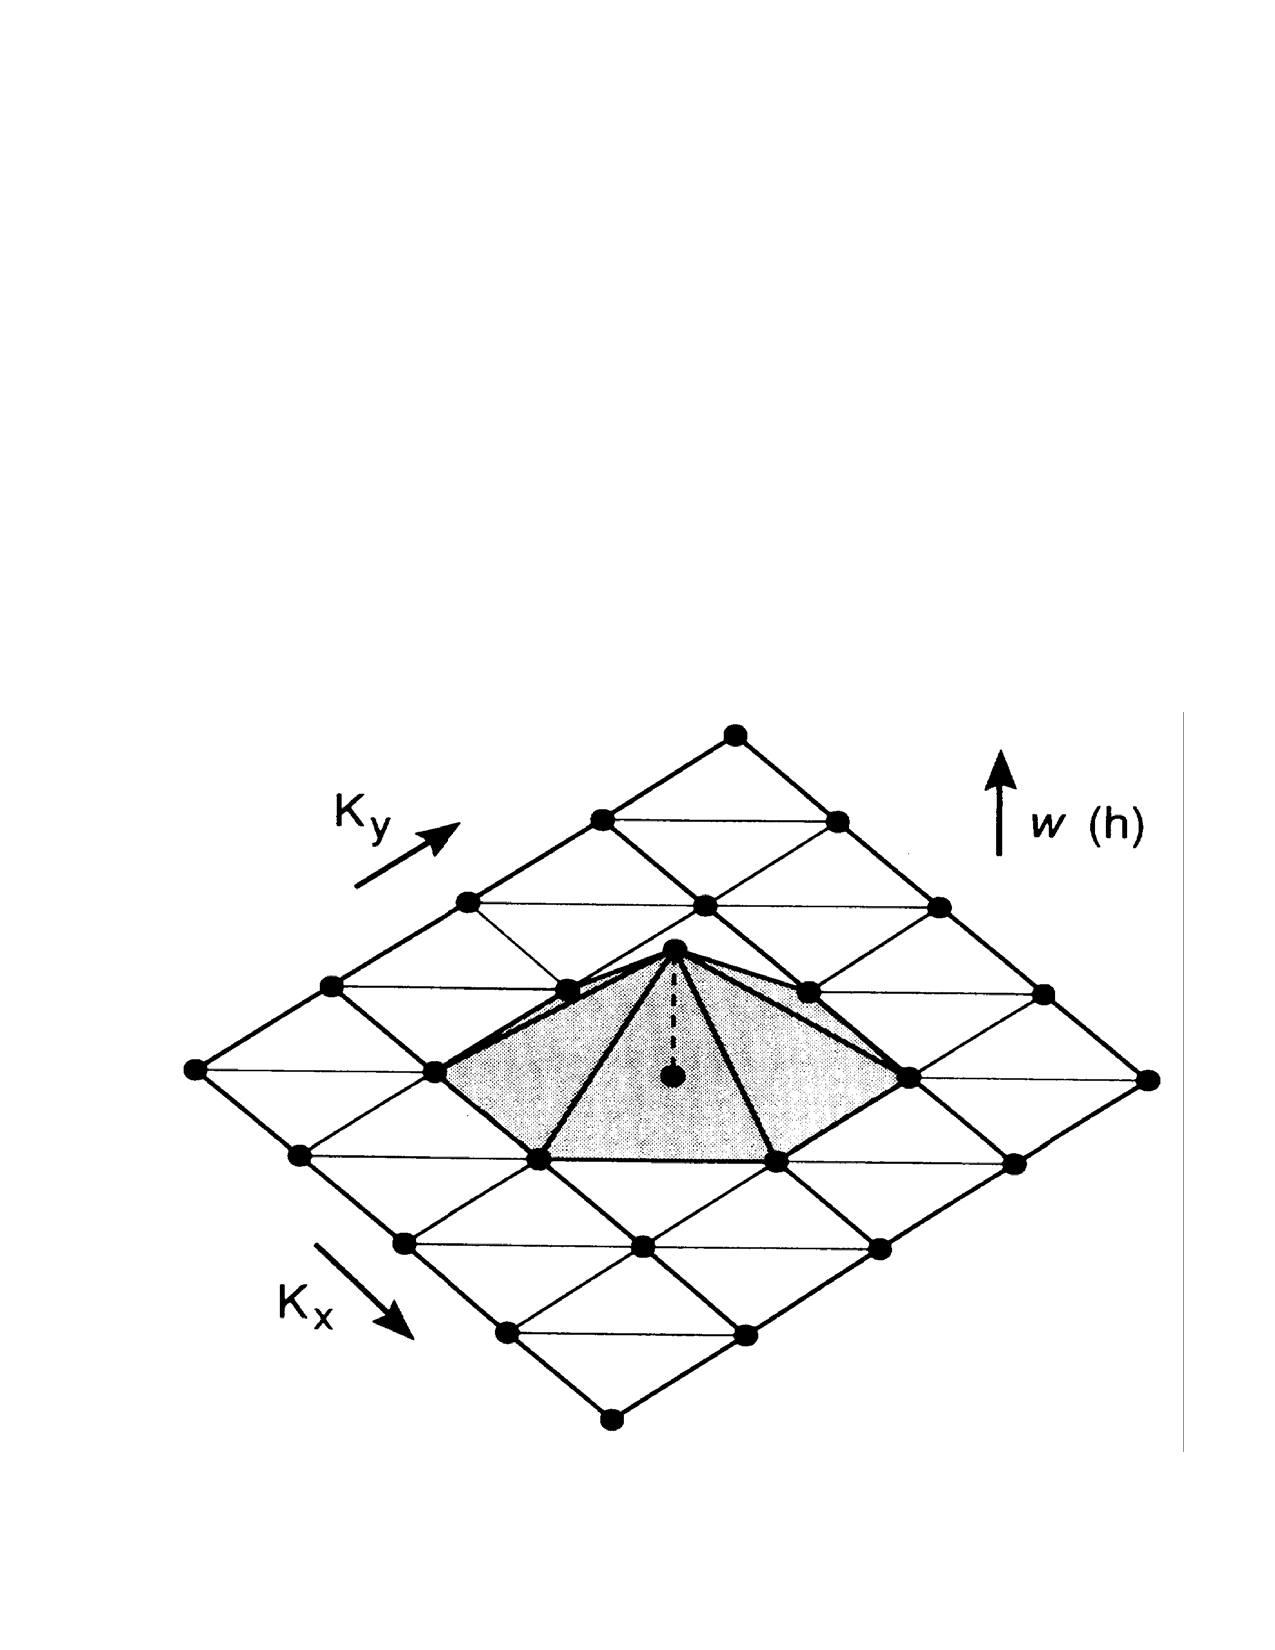
\includegraphics[height=2.75in,width=3.05in,viewport=0 30 565 505,clip]{Figures/dimen_Tetra.pdf}
%\caption{\small Two-dimensional schematic illustration of the function $w_j(\vec k)$.}%(与文献\cite{EPJB33-47_2003}图1对比)
%\label{Fig:Submesh_Tetra}
%\end{figure}
%}

\appendix
\frame
{
	\frametitle{四面体对\textrm{DOS}的贡献}
	类似地,可以确定每个四面体对态密度(\textrm{DOS})$D_T(\varepsilon)$的贡献,计算方案如下
	\begin{itemize}
	\item $\varepsilon<\varepsilon_1$
		\begin{displaymath}
			D_T(\varepsilon)=0
		\end{displaymath}
	\item $\varepsilon_1<\varepsilon<\varepsilon_2$
		\begin{displaymath}
			D_T(\varepsilon)=\dfrac{V_T}{V_G}\dfrac{3(\varepsilon-\varepsilon_1)^2}{\varepsilon_{21}\varepsilon_{31}\varepsilon_{41}}
		\end{displaymath}
	\item $\varepsilon_2<\varepsilon<\varepsilon_3$
		\begin{displaymath}
			\hspace*{-25pt}	D_T(\varepsilon)=\dfrac{V_T}{V_G}\dfrac1{\varepsilon_{31}\varepsilon_{41}}\left[3\varepsilon_{21}+6(\varepsilon-\varepsilon_2)-3\dfrac{(\varepsilon_{31}+\varepsilon_{42})(\varepsilon-\varepsilon_2)^2}{\varepsilon_{32}\varepsilon_{42}}\right]
		\end{displaymath}
	\item $\varepsilon_3<\varepsilon<\varepsilon_4$
		\begin{displaymath}
			D_T(\varepsilon)=\dfrac{V_T}{V_G}\dfrac{3(\varepsilon_4-\varepsilon)^2}{\varepsilon_{41}\varepsilon_{42}\varepsilon_{43}}
		\end{displaymath}
	\item $\varepsilon>\varepsilon_4$
		\begin{displaymath}
			D_T(\varepsilon)=0
		\end{displaymath}
	\end{itemize}
}
%------------------------------------------------------------------------Reference----------------------------------------------------------------------------------------------
%\begin{thebibliography}{99}
%-----------------------------------------------------------------------------------------------------------------------------------------------------------------------%
%\frame
%{
%\frametitle{主要参考文献}
%{\small
%\bibitem{Singh_Book}\textrm{D. J. Singh. \textit{Plane Wave, PseudoPotential and the LAPW method} (Kluwer Academic, Boston,USA, 1994)}					%
%  \nocite{*}																				%
%}
%}
%\end{thebibliography}

\begin{thebibliography}{99}
\frame
{
\frametitle{主要参考文献}
{\small
%	\bibitem{Huang_Han}黄昆\:原著、韩汝琦\:改编, {\textit{固体物理学}}\:高等教育出版社, 北京, 1988
%	\bibitem{Xie_Lu}谢希德、陆栋\:主编, {\textit{固体能带理论}}\:复旦大学出版社, 上海, 1998
	\bibitem{PRB40-3616_1989}\textrm{M. Methfessel and A. T. Paxton \textit{Phys. Rev.} B, \textbf{40} (1989), 3616}
	\bibitem{PRB49-16223_1994}\textrm{P. E. Bl\"ochl, O. Jepsen and O. K. Andersen \textit{Phys. Rev.} B, \textbf{49} (1994), 16223}
}
\nocite*{}
}
\end{thebibliography}
%{\small
%\phantomsection\addcontentsline{toc}{section}{Bibliography}	 %直接调用\addcontentsline命令可能导致超链指向不准确,一般需要在之前调用一次\phantomsection命令加以修正	%
%\bibliography{Myref}																			%
%\bibliographystyle{mybib}																		%
%  \nocite{*}																				%
%}
%-----------------------------------------------------------------------------------------------------------------------------------------------------------------------%


%-----------------------------------------------------------Beamer下不建议使用bib,因为涉及分页--------------------------------------------------------------------------%
%{\small
%\phantomsection\addcontentsline{toc}{section}{Bibliography}	 %直接调用\addcontentsline命令可能导致超链指向不准确,一般需要在之前调用一次\phantomsection命令加以修正	%
%\bibliography{Myref}																			%
%\bibliographystyle{mybib}																		%
%  \nocite{*}																				%
%}

%------------------------------------------------------------------------------------------------------------------------------------------------------------------------------%

%-------------------------------------------------------------------------Thanks------------------------------------------------------------------------------------------------
%\section{致谢}
%\frame
%{
%\frametitle{致$\quad$谢}
%\begin{itemize}
%    \setlength{\itemsep}{20pt}
%  \item 感谢本团队高兴誉、吴泉生、宋红州等各位老师参与的讨论
%  \item 感谢莫所长、宋主任以及软件中心各位老师和同事
%  \item 感谢王崇愚先生的帮助
%\end{itemize}
%}

\logo{}									%不显示logo
\frame
{
\vskip 60 pt
%\hskip 10pt \textcolor{blue}{\Huge 感谢答辩委员会各位老师\,\textrm{!}}\\
\vskip 35 pt
\hskip 60pt \textcolor{blue}{\Huge 谢谢大家\:!}
%\vskip 15 pt
%\hskip 40pt \textcolor{blue}{\Huge \textrm{for your attention\:!}}
}

%-------------------------------------------------------------------------------------------------------------------------------------------------------------------------------

\clearpage
%\end{CJK*}
\end{document}
